%! ~~~ Packages Setup ~~~ 
\documentclass[]{article}


% Math packages
\usepackage[usenames]{color}
\usepackage{forest}
\usepackage{ifxetex,ifluatex,amsmath,amssymb,mathrsfs,amsthm,witharrows,mathtools}
\WithArrowsOptions{displaystyle}
\renewcommand{\qedsymbol}{$\blacksquare$} % end proofs with \blacksquare. Overwrites the defualts. 
\usepackage{cancel,bm}
\usepackage[thinc]{esdiff}


% tikz
\usepackage{tikz}
\usetikzlibrary{decorations.pathreplacing} % Importing the decoration library for braces
\newcommand\sqw{1}
\newcommand\squ[4][1]{\fill[#4] (#2*\sqw,#3*\sqw) rectangle +(#1*\sqw,#1*\sqw);}


% code 
\usepackage{listings}
\usepackage{xcolor}

\definecolor{codegreen}{rgb}{0,0.35,0}
\definecolor{codegray}{rgb}{0.5,0.5,0.5}
\definecolor{codenumber}{rgb}{0.1,0.3,0.5}
\definecolor{codeblue}{rgb}{0,0,0.5}
\definecolor{codered}{rgb}{0.5,0.03,0.02}
\definecolor{codegray}{rgb}{0.96,0.96,0.96}

\lstdefinestyle{pythonstylesheet}{
	language=Python,
	emphstyle=\color{deepred},
	backgroundcolor=\color{codegray},
	keywordstyle=\color{deepblue}\bfseries\itshape,
	numberstyle=\scriptsize\color{codenumber},
	basicstyle=\ttfamily\footnotesize,
	commentstyle=\color{codegreen}\itshape,
	breakatwhitespace=false, 
	breaklines=true, 
	captionpos=b, 
	keepspaces=true, 
	numbers=left, 
	numbersep=5pt, 
	showspaces=false,                
	showstringspaces=false,
	showtabs=false, 
	tabsize=4, 
	morekeywords={as,assert,nonlocal,with,yield,self,True,False,None,AssertionError,ValueError,in,else},              % Add keywords here
	keywordstyle=\color{codeblue},
	emph={object,type,isinstance,copy,deepcopy,zip,enumerate,reversed,list,set,len,dict,tuple,print,range,xrange,append,execfile,real,imag,reduce,str,repr,__init__,__add__,__mul__,__div__,__sub__,__call__,__getitem__,__setitem__,__eq__,__ne__,__nonzero__,__rmul__,__radd__,__repr__,__str__,__get__,__truediv__,__pow__,__name__,__future__,__all__,},          % Custom highlighting
	emphstyle=\color{codered},
	stringstyle=\color{codegreen},
	showstringspaces=false,
	abovecaptionskip=0pt,belowcaptionskip =0pt,
	framextopmargin=-\topsep, 
}
\newcommand\pythonstyle{\lstset{pythonstylesheet}}
\newcommand\pyl[1]     {{\lstinline!#1!}}
\lstset{style=pythonstylesheet}

\usepackage[style=1,skipbelow=\topskip,skipabove=\topskip,framemethod=TikZ]{mdframed}
\definecolor{bggray}{rgb}{0.85, 0.85, 0.85}
\mdfsetup{leftmargin=0pt,rightmargin=0pt,innerleftmargin=15pt,backgroundcolor=codegray,middlelinewidth=0.5pt,skipabove=5pt,skipbelow=0pt,middlelinecolor=black,roundcorner=5}
\BeforeBeginEnvironment{lstlisting}{\begin{mdframed}\vspace{-0.4em}}
	\AfterEndEnvironment{lstlisting}{\vspace{-0.8em}\end{mdframed}}


% Deisgn
\usepackage[labelfont=bf]{caption}
\usepackage[margin=0.4in]{geometry}
\usepackage{multicol}
\usepackage[skip=4pt, indent=0pt]{parskip}
\usepackage[normalem]{ulem}
\forestset{default}
\renewcommand\labelitemi{$\bullet$}
\usepackage{titlesec}
\titleformat{\section}[block]
	{\fontsize{18}{18}}
	{\Large \dotfill \ (\thesection) \dotfill}
	{0em}
	{\vspace{6pt} \newline \hfil \Large \filleft \filright \MakeUppercase}

\graphicspath{ {./} }
\newtheorem{theorem}{Theorem}[section]
\newtheorem{definition}{Definition}[section]


% Language Shortcuts
\newcommand\en[1] {\begin{otherlanguage}{english}#1\end{otherlanguage}}
\newcommand\sen   {\begin{otherlanguage}{english}}
	\newcommand\she   {\end{otherlanguage}}
\newcommand\del   {$ \!\! $}
\newcommand\ttt[1]{\en{\footnotesize\texttt{#1}\normalsize}}

\newcommand\npage {\vfil {\hfil \textbf{\textit{המשך בעמוד הבא}}} \hfil \vfil \pagebreak}
\newcommand\ndoc  {\dotfill \\ \vfil {\begin{center} {\textbf{\textit{שחר פרץ, 2024}} \\ \scriptsize \textit{נוצר באמצעות תוכנה חופשית בלבד}} \end{center}} \vfil	}

\newcommand{\rn}[1]{
	\textup{\uppercase\expandafter{\romannumeral#1}}
}

\makeatletter
\newcommand{\skipitems}[1]{
	\addtocounter{\@enumctr}{#1}
}
\makeatother

%! ~~~ Math shortcuts ~~~

% Letters shortcuts
\newcommand\N     {\mathbb{N}}
\newcommand\Z     {\mathbb{Z}}
\newcommand\R     {\mathbb{R}}
\newcommand\Q     {\mathbb{Q}}
\newcommand\C     {\mathbb{C}}

\newcommand\ml    {\ell}
\newcommand\mj    {\jmath}
\newcommand\mi    {\imath}

\newcommand\powerset {\mathcal{P}}
\newcommand\ps    {\mathcal{P}}
\newcommand\pc    {\mathcal{P}}
\newcommand\ac    {\mathcal{A}}
\newcommand\bc    {\mathcal{B}}
\newcommand\cc    {\mathcal{C}}
\newcommand\dc    {\mathcal{D}}
\newcommand\ec    {\mathcal{E}}
\newcommand\fc    {\mathcal{F}}
\newcommand\nc    {\mathcal{N}}
\newcommand\sca   {\mathcal{S}} % \sc is already definded
\newcommand\rca   {\mathcal{R}} % \rc is already definded

\newcommand\Si    {\Sigma}

% Logic & sets shorcuts
\newcommand\siff  {\longleftrightarrow}
\newcommand\ssiff {\leftrightarrow}
\newcommand\so    {\longrightarrow}
\newcommand\sso   {\rightarrow}

\newcommand\epsi  {\epsilon}
\newcommand\vepsi {\varepsilon}
\newcommand\vphi  {\varphi}
\newcommand\Neven {\N_{\mathrm{even}}}
\newcommand\Nodd  {\N_{\mathrm{odd }}}
\newcommand\Zeven {\Z_{\mathrm{even}}}
\newcommand\Zodd  {\Z_{\mathrm{odd }}}
\newcommand\Np    {\N_+}

% Text Shortcuts
\newcommand\open  {\big(}
\newcommand\qopen {\quad\big(}
\newcommand\close {\big)}
\newcommand\also  {\text{, }}
\newcommand\defi  {\text{ definition}}
\newcommand\defis {\text{ definitions}}
\newcommand\given {\text{given }}
\newcommand\case  {\text{if }}
\newcommand\syx   {\text{ syntax}}
\newcommand\rle   {\text{ rule}}
\newcommand\other {\text{else}}
\newcommand\set   {\ell et \text{ }}
\newcommand\ans   {\mathit{Ans.}}

% Set theory shortcuts
\newcommand\ra    {\rangle}
\newcommand\la    {\langle}

\newcommand\oto   {\leftarrow}

\newcommand\QED   {\quad\quad\mathscr{Q.E.D.}\;\;\blacksquare}
\newcommand\QEF   {\quad\quad\mathscr{Q.E.F.}}
\newcommand\eQED  {\mathscr{Q.E.D.}\;\;\blacksquare}
\newcommand\eQEF  {\mathscr{Q.E.F.}}
\newcommand\jQED  {\mathscr{Q.E.D.}}

\newcommand\dom   {\mathrm{dom}}
\newcommand\Img   {\mathrm{Im}}
\newcommand\range {\mathrm{range}}

\newcommand\trio  {\triangle}

\newcommand\rc    {\right\rceil}
\newcommand\lc    {\left\lceil}
\newcommand\rf    {\right\rfloor}
\newcommand\lf    {\left\lfloor}

\newcommand\lex   {<_{lex}}

\newcommand\az    {\aleph_0}
\newcommand\uaz   {^{\aleph_0}}
\newcommand\al    {\aleph}
\newcommand\ual   {^\aleph}
\newcommand\taz   {2^{\aleph_0}}
\newcommand\utaz  { ^{\left (2^{\aleph_0} \right )}}
\newcommand\tal   {2^{\aleph}}
\newcommand\utal  { ^{\left (2^{\aleph} \right )}}
\newcommand\ttaz  {2^{\left (2^{\aleph_0}\right )}}

\newcommand\n     {$n$־יה\ }

% Math A&B shortcuts
\newcommand\logn  {\log n}
\newcommand\logx  {\log x}
\newcommand\lnx   {\ln x}
\newcommand\cosx  {\cos x}
\newcommand\cost  {\cos \theta}
\newcommand\sinx  {\sin x}
\newcommand\sint  {\sin \theta}
\newcommand\tanx  {\tan x}
\newcommand\tant  {\tan \theta}
\newcommand\sex   {\sec x}
\newcommand\sect  {\sec^2}
\newcommand\cotx  {\cot x}
\newcommand\cscx  {\csc x}
\newcommand\sinhx {\sinh x}
\newcommand\coshx {\cosh x}
\newcommand\tanhx {\tanh x}

\newcommand\seq   {\overset{!}{=}}
\newcommand\slh   {\overset{LH}{=}}
\newcommand\sle   {\overset{!}{\le}}
\newcommand\sge   {\overset{!}{\ge}}
\newcommand\sll   {\overset{!}{<}}
\newcommand\sgg   {\overset{!}{>}}

\newcommand\ve    {\vec}
\newcommand\lv    {\overrightarrow}
\newcommand\ol    {\overline}

\newcommand\mlcm  {\mathrm{lcm}}

\DeclareMathOperator{\sech}   {sech}
\DeclareMathOperator{\csch}   {csch}
\DeclareMathOperator{\arcsec} {arcsec}
\DeclareMathOperator{\arccot} {arcCot}
\DeclareMathOperator{\arccsc} {arcCsc}
\DeclareMathOperator{\arccosh}{arccosh}
\DeclareMathOperator{\arcsinh}{arcsinh}
\DeclareMathOperator{\arctanh}{arctanh}
\DeclareMathOperator{\arcsech}{arcsech}
\DeclareMathOperator{\arccsch}{arccsch}
\DeclareMathOperator{\arccoth}{arccoth}
\DeclareMathOperator{\atant}  {atan2} 

\newcommand\h     {\text{\!\footnotesize$[h]$\normalsize}}

\newcommand\dx    {\,\mathrm{d}x}
\newcommand\dt    {\,\mathrm{d}t}
\newcommand\dtt   {\,\mathrm{d}\theta}
\newcommand\du    {\,\mathrm{d}u}
\newcommand\dv    {\,\mathrm{d}v}
\newcommand\df    {\mathrm{d}f}
\newcommand\dfdx  {\diff{f}{x}}
\newcommand\dit   {\limhz \frac{f(x + h) - f(x)}{h}}

\newcommand\nt[1] {\frac{#1}{#1}}

\newcommand\limz  {\lim_{x \to 0}}
\newcommand\limxz {\lim_{x \to x_0}}
\newcommand\limi  {\lim_{x \to \infty}}
\newcommand\limh  {\lim_{x \to 0}}
\newcommand\limni {\lim_{x \to - \infty}}
\newcommand\limpmi{\lim_{x \to \pm \infty}}

\newcommand\ta    {\theta}
\newcommand\ap    {\alpha}

\renewcommand\inf {\infty}
\newcommand  \ninf{-\inf}

% Combinatorics shortcuts
\newcommand\sumnk     {\sum_{k = 0}^{n}}
\newcommand\sumni     {\sum_{i = 0}^{n}}
\newcommand\sumnko    {\sum_{k = 1}^{n}}
\newcommand\sumnio    {\sum_{i = 1}^{n}}
\newcommand\sumai     {\sum_{i = 1}^{n} A_i}
\newcommand\nsum[2]   {\reflectbox{\displaystyle\sum_{\reflectbox{\scriptsize$#1$}}^{\reflectbox{\scriptsize$#2$}}}}

\newcommand\bink      {\binom{n}{k}}
\newcommand\setn      {\{a_i\}^{2n}_{i = 1}}
\newcommand\setc[1]   {\{a_i\}^{#1}_{i = 1}}

\newcommand\cupain    {\bigcup_{i = 1}^{n} A_i}
\newcommand\cupai[1]  {\bigcup_{i = 1}^{#1} A_i}
\newcommand\cupiiai   {\bigcup_{i \in I} A_i}
\newcommand\capain    {\bigcap_{i = 1}^{n} A_i}
\newcommand\capai[1]  {\bigcap_{i = 1}^{#1} A_i}
\newcommand\capiiai   {\bigcap_{i \in I} A_i}

\newcommand\xot       {x_{1, 2}}
\newcommand\ano       {a_{n - 1}}
\newcommand\ant       {a_{n - 2}}

% Other shortcuts
\newcommand\tl    {\tilde}
\newcommand\op    {^{-1}}

\newcommand\sof[1]    {\left | #1 \right |}
\newcommand\cl [1]    {\left ( #1 \right )}
\newcommand\csb[1]    {\left [ #1 \right ]}

\newcommand\bs    {\blacksquare}

%! ~~~ Document ~~~

\author{Shahar Perets}
\title{Course B $\sim$ Shit Cheat Sheet}
\begin{document}
	\begin{multicols}{2}
		
		
		\section{General}
		
		\begin{definition}
			$\R[x]$ is the group of all polynomials with real coefficients. 
		\end{definition}
		
		\begin{theorem}
			$\forall p(x) \in \R[x]. \forall z \in \C. p(z) = 0 \iff p(\bar z)$
		\end{theorem}
		
		\begin{definition}
			$\C[x]$ is the group of all polynomials with complex coefficient. 
		\end{definition}
		
		\begin{theorem}
			$p(x_0) = 0 \iff (x - x_0) \mid p(x_0)$
		\end{theorem}
		
		\begin{theorem}[Fundamental theorem of algebra]
			For all $p(x) \in \C$ non-constant, exists $z \in \C$ such as $p(z) = 0$. 
		\end{theorem}
		
		\begin{theorem}[The Politics Assumption]
			A problem is dismissed iff it would be became bigger problem in the future. 
		\end{theorem}
		
		\begin{theorem}[Snell's Law]
			Given $v_1, v_2$ speeds to pass $y_1, y_2$ repectively;
			\begin{center}
				\footnotesize
				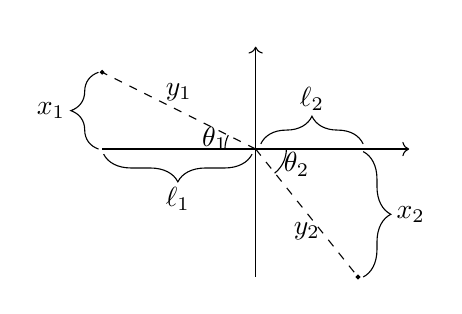
\begin{tikzpicture}[scale=0.65]
					% Axis
					\draw[thin,->] (-3,0) -- (3,0) node[right] {};
					\draw[thin,->] (0,-2.5) -- (0,2) node[above] {};
					% Lines l1 and l2
					\draw[dashed] (0, 0) -- (-3,1.5) node[right] {}; % l1
					\draw[dashed] (0, 0) -- (2,-2.5) node[right] {}; % l2
					% Coordinates on the axis
					\draw[fill=black] (-3,1.5) circle (1pt); % Point on l1
					\draw[fill=black] (2,-2.5) circle (1pt); % Point on l2
					\draw[fill=black] (-1.5, 0.75) circle (0pt) node[above] {$y_1$};
					\draw[fill=black] (1, -1.25) circle (0pt) node[below] {$y_2$};
					% Braces for x1 and x2
					\draw[decorate,decoration={brace,amplitude=10pt},xshift=-2pt,yshift=0cm] (-3,0) -- (-3,1.5) node[midway,left=0.3cm] {$x_1$};
					\draw[decorate,decoration={brace,amplitude=10pt},xshift=0.1cm,yshift=-0.05cm] (2,0) -- (2,-2.45) node[midway,right=0.3cm] {$x_2$};
					% Braces for l1 and l2
					\draw[decorate,decoration={brace,amplitude=10pt},xshift=-2pt,yshift=-0.1cm] (0,0) -- (-2.9,0) node[midway,below=0.3cm] {$\ell_1$};
					\draw[decorate,decoration={brace,amplitude=10pt},xshift=0.1cm,yshift=0.1cm] (0,0) -- (2,0) node[midway,above=0.3cm] {$\ell_2$};
					% Angle theta_1
					\draw[] (-0.6,0) arc[start angle=180, end angle=153, radius=0.6];
					\node at (-0.8,0.2) {$\theta_1$};
					% Angle theta_2
					\draw[] (0.6,0) arc[start angle=0, end angle=-52, radius=0.6];
					\node at (0.8,-0.3) {$\theta_2$};
				\end{tikzpicture}
				\normalsize
			\end{center}
			We denote $d = x_1 + x_2$. We get that: 
			\[ \theta_2 = \arctan\cl{\frac{d - \ml_1\tan\theta_1}{\ml_2}} \]
			Hence, when $t$ is the time required to get from one point to another with the given speeds: 
			\[ t(\theta_1) = \frac{\ell_1}{v_1\cos\ta_1} + \frac{\ell_1}{v_2}\sqrt{1 + \cl{\frac{\ell_1\tan\ta_1 - d}{\ml_2}}^2} \]
			And $t$ is minimal when: 
			\[ \frac{\sin\ta_1}{v_1} = \frac{\sin\ta_2}{v_2} \]	
		\end{theorem}
		
		
		
		\section{Limits etc.}
		
		\begin{definition}[Dirichlet function]
			\[ D(x) \equiv \begin{cases}
				1 & x \in \Q \\
				0 & x \in \R
			\end{cases} = \mathbf{1}_\Q \]
		\end{definition}
		
		\begin{theorem}
			Assuming $\limxz f(x) = L_f $ and $\limxz g(x) = L_g$ where $L_f, L_g \in \R \lor L_f = L_g = \pm\inf$, then $\limxz f + g = L_f + L_g$, and $\limxz f \cdot g = L_fL_g$. 
		\end{theorem}
		
		\begin{definition}
			A function $f(x) \in \R \to \R$ is continues in $x_0$ iff $\limxz f(x_0) = f(x_0)$. 
		\end{definition}
		
		\begin{definition}
			$f \in I \to \R$ has the intermediate value property iff $\forall a, b \in I. \exists c \in [a, b]. f(c) \in [f(a), f(b)]$. 
		\end{definition}
		
		\begin{theorem}[Intermediate value theorem]
			If $f \in I \to \R$ is continues, then $f$ has the intermediate value property. 
		\end{theorem}
		
		\begin{theorem}
			If $\limxz f(x) = \limxz h(x) = L$ and $\forall x \in [a, b] \neq \emptyset. f(x) \le g(x) \le h(x) \land x_0 \in [a, b]$, then $\limxz g(x) = L$. 
		\end{theorem}
		
		\begin{theorem}[Lhopital rule]
		Assuming $\limxz f'(x) = L_f, \limxz g'(x) = L_g$ both exists, then: 
		\[ \limxz \frac{f(x)}{g(x)} = \frac{L_f}{L_g} \]
		\end{theorem}
		
		\begin{theorem}
			Where $ f\op $ is the inverse function of $f$ for a given interval;
			\[ f\op{'} = \frac{1}{f'f(\op)} \]
		\end{theorem}
		
		
		
		\section{Trigo and Hypr-Trigo}
		
		\begin{definition}[Hyperbolic functions]
			\[ \coshx = \frac{e^x + e^{-x}}{2}, \ \sinhx = \frac{e^x - e^{-x}}{2} \]
		\end{definition}
		
		\begin{theorem}
			\begin{gather*}
				\cosh^2x - \sinh^2x = 1, \\
				\sinh(x + y) = \sinh y \coshx + \sinhx \cosh y, \\ 
			\end{gather*}
		\end{theorem}
		
		\begin{theorem}
			\[ \arccosh = \ln(x + \sqrt{x^2 - 1}), \ \arcsinh = \ln(x + \sqrt{x^2 + 1}) \]
		\end{theorem}
		
		\begin{theorem}
			We denote $\pm = +$ for trigonometric functions, and $\pm = -$ for hyperbolic functions. $\mp$ is the inverse of $\pm$.
			\begin{alignat*}{9}
				\arcsin\h &= \sec\h(\arcsin\h) &&= \frac{1}{\sqrt{1 \mp x^2}} \\
				\arccos\h &= \mp\csc\h(\arcsin\h) &&= \mp \frac{1}{\sqrt{x^2 - 1}} \\
				\arctan\h &= \cos\h^2(\arctan\h) &&= \frac{1}{1 \pm x^2}
			\end{alignat*}
		\end{theorem}
		
		
		
		\section{Derivatives}
		
		\begin{definition}[implicit diffrentiation]
			diffrentiating both sides of the equation. E.g.: 
			\[ y = f(x), \ xf(x) = 1 \to f(x) + f'(x)x = 1' = 0 \to y' = -\frac{y}{x} \]
		\end{definition}
		
		\begin{definition}
			\[ e_n \equiv \cl{1 + \frac{1}{n}}^n \]
		\end{definition}
		
		\begin{theorem}
			$e_n$ is monotonically increasing
		\end{theorem}
		
		\begin{definition}
			\[ e \equiv \limi \cl{1 + \frac{1}{n}}^{n} \]
		\end{definition}
		
		\begin{theorem}
			\begin{gather*}
				f(x) = \log_ax \implies f'(x) = \frac{1}{x\ln a} \\
				f(x) = a^x \implies f'(x) = \ln a \cdot a^{x}
			\end{gather*}
		\end{theorem}
		
		\begin{theorem}
			\[ \exists I \ \mathrm{interval}. \forall x \in I. f'(x) = f(x) \implies \exists c \in \R. f(x) = ce^x \]
		\end{theorem}
		
		\begin{theorem}[Darbuax Theorm]
			If $f$ diffrentiatable in $I \subseteq \R$, then $f'$ has the intermediate value property. 
		\end{theorem}
		
		
		
		\section{Integrals}
		
		\begin{definition}
			$F(x)$ is an antiderivative of $f(x)$ if $F'(x) = f(x)$. 
		\end{definition}
		
		\begin{theorem}
			If $F_1, F_2$ antiderivatives of $f$ in $I \subseteq \R$, then exists $C \in \R$ such as $F_1 - F_2 = C$. 
		\end{theorem}
		
		\begin{theorem}
			\begin{gather*}
				\int (f + g)\dx = \int f\dx + \int g \dx = F + G + C \\
				\int af(x) \dx = a \int f(x)\dx = aF(x) + C \\
				\int f(ax + b)\dx  = \frac{1}{a} F(ax + b) + C
			\end{gather*}
		\end{theorem}
		
		\begin{theorem}
			\[ \int f(t(x))t'(x)\dx = \int f(t)\dt \]
		\end{theorem}
		
		\begin{theorem}[Lagrange's mean value theorem]
			Let $F$ be an antiderivative of $f$ in $[c, d]$. Then exists $c \le x \le d$ such as: 
			\[ f(x) = \frac{F(d) - F(c)}{c - d} \]
		\end{theorem}
		
		\begin{theorem}[Fundamental theorem of calc]
			\[ S = \int^b_a f(x)\dx = F(b) - F(a) \]
			Where $S$ is the area under $f(x)$ in range $[a, b]$. 
		\end{theorem}
		
		\begin{theorem}
			\[ \int^a_b f(x) \dx = -\int^b_a f(x) \dx \]
		\end{theorem}
		
		\begin{theorem}[Integration by parts (IBP)]
			\[ \int u\dv = uv - \int v\du \]
		\end{theorem}
		
		
		\section{Taylow Series}
		
		\begin{definition}[Taylow Series]
			Taylow series around $x_0 \in \R$ for $f \in \R^\R$ is: 
			\[ \sum_{k = 0}^{\inf}\frac{f^{(n)}(x_0)}{k!}(x - x_0)^k \]
		\end{definition}
		
		\begin{theorem}
			The taylor series for $f(x)$ is equal to $f(x)$ for "many functions". 
		\end{theorem}
		
		\begin{definition}[Maclaurin Series] is taylor series around $0$:
			\[ \sum_{n = 0}^{\inf}\frac{f^{(n)}(0)}{n!}x^n \]
		\end{definition}
		
		\begin{theorem}[Maclaurin Series for common functions]
			\begin{alignat*}{9}
				\sinx &= \sum_{k = 0}^{\inf}\frac{(-1)^k}{(2k + 1)!}x^{2k + 1} \\
				\cosx &= \sum_{k = 0}^{\inf}\frac{(-1)^k}{(2k)!}x^{2k} \\
				e^x &= \sum_{k = 0}^{\inf}\frac{x^k}{k!} \\
				\frac{1}{x} &= \sum_{m = 0}^{\inf}-(x + 1)^m && \quad [-2 \le x \le 0] \\
				\ln(1 - x) &= \sum_{k = 0}^{\inf} -\frac{x^k}{k}
			\end{alignat*}
			Note that Maclaurin Series for $e^{-\frac{1}{x^2}}$ equals $0$. 
		\end{theorem}
		
		\begin{theorem}[Weierstrass Substitution]
			$\set t = \tan \frac{x}{2}$;
			\[ \int f(\sinx, \cosx \dx)\dx =\!\! \int f \cl{\frac{2t}{1 + t^2}, \frac{1 - t^2}{1 + t^2}}\frac{2\dt}{1 + t^2}\dt \]
		\end{theorem}
		
		
		\section{Complex Numbers}
		
		\begin{definition}
			For $z \in \C$, $\sin z, \cos z$ and $e^z$ is defined to be the result of the Maclaurin Series' output for $z$. 
		\end{definition}
		
		\begin{theorem}
			\[\forall x, y \in \C, e^{x + y} = e^x + e^y\]
		\end{theorem}
		
		\begin{theorem}[Euler Formula]
			\[ \forall x \in \C. \ e^{ix} = \cosx + i\sinx \]
		\end{theorem}
		
		Hence, for all $\C \ni x = a + bi = \Re(x) + \Im(x)i$ where $a, b \in \R$, we know that $r \equiv |e^x| = e^{\Re(x)}$ and the angle of $e^x$ is $b$. To summrize: 
		
		\begin{theorem}
			\[ z = r(\cos\theta + i\sin\theta) = e^{\ln r + i\theta} = re^{i\theta} \]
		\end{theorem}
		
		\begin{theorem}
			\[ z^n = r^n(\sin\theta + i\cos\theta) \]
		\end{theorem}
		
		\begin{theorem}
			\begin{gather*}
				u_n := \cos\cl{\frac{2\pi}{n}} + i\sin\cl{\frac{2n}{n}} \\ \forall n \in \N. z \in \{u^{m} \mid m \in \N\} \iff z^n = 1
			\end{gather*}
		\end{theorem}
		
	\end{multicols}
	
	\dotfill{\Large \ \textbf{I may have some mistakes}\ }\dotfill
	{\let\newpage\relax\maketitle}
\end{document}